\usetikzlibrary{arrows.meta}
\tikzset{%
  >={Latex[width=2mm,length=2mm]},
  % Specifications for style of nodes:
            base/.style = {rectangle, rounded corners, draw=black,
                           minimum width=6cm, minimum height=1cm,
                           text centered, font=\sffamily},
  activityStarts/.style = {base, fill=blue!30},
}

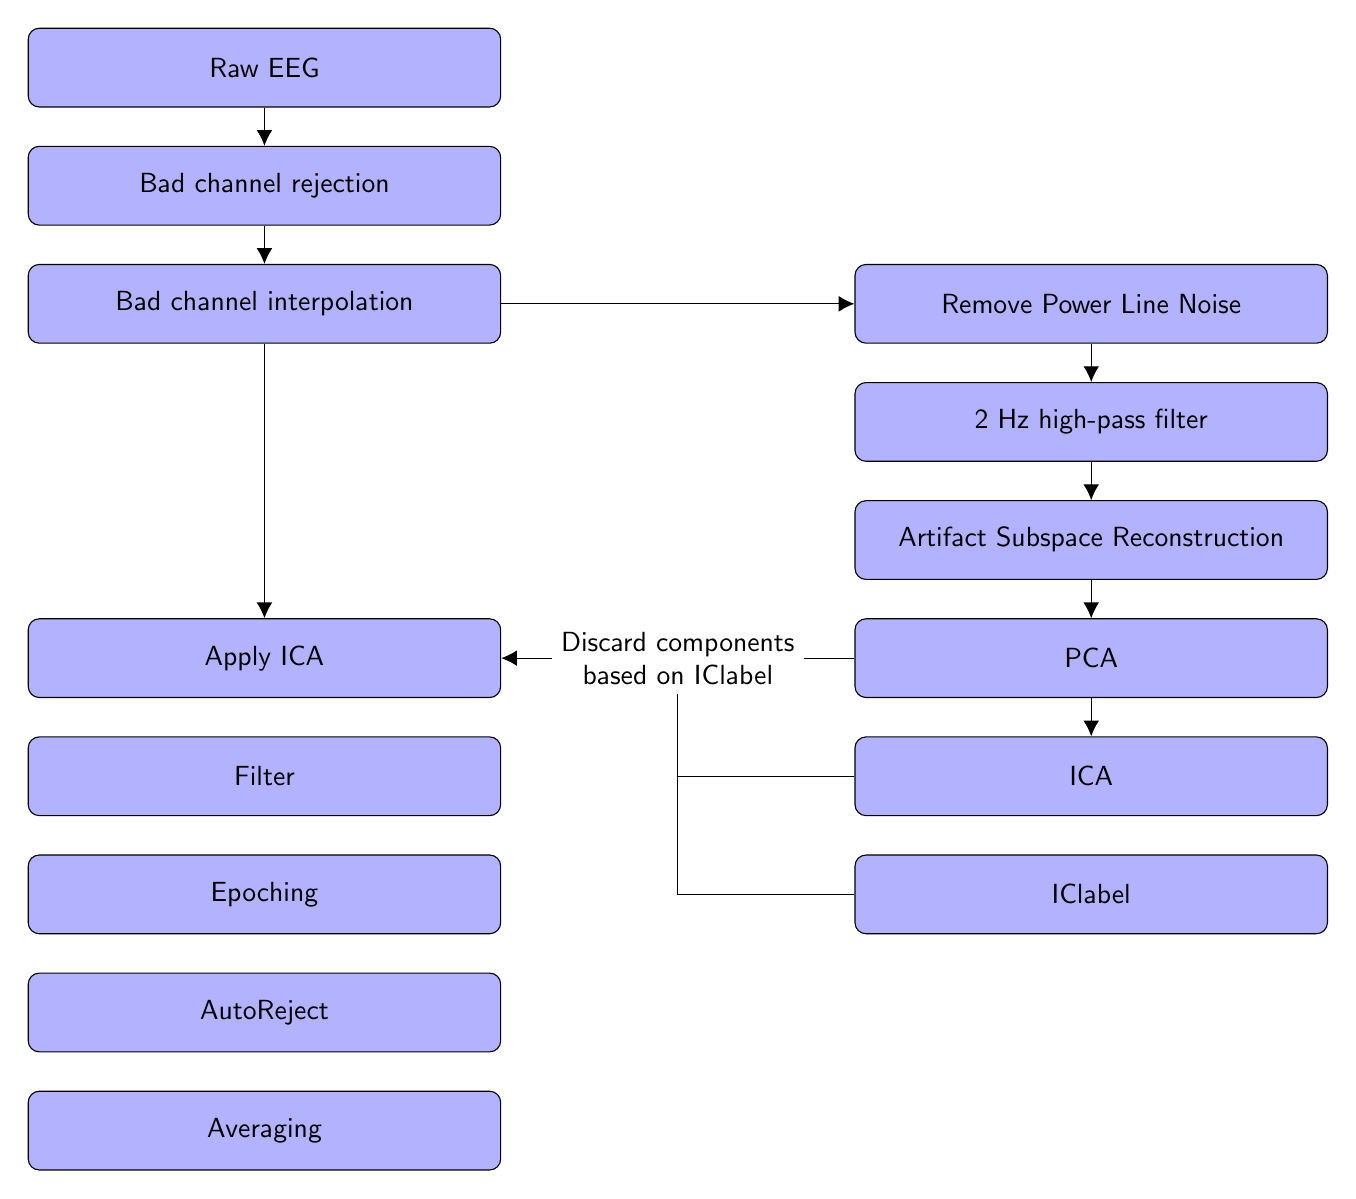
\begin{tikzpicture}[node distance=1.5cm,
    every node/.style={fill=white, font=\sffamily}, align=center]
  % Specification of nodes (position, etc.)
  \node (raw)             [activityStarts]                    {Raw EEG};
  \node (badchannels)     [activityStarts, below of=raw]   {Bad channel rejection};
  \node (interpolation)     [activityStarts, below of=badchannels]   {Bad channel interpolation};
  
  \node (zapline)       [activityStarts, right of=interpolation, xshift=9cm]   {Remove Power Line Noise};
  \node (icafilter)       [activityStarts, below of=zapline]   {2 Hz high-pass filter};
  \node (asr)       [activityStarts, below of=icafilter]   {Artifact Subspace Reconstruction};
  \node (pca)       [activityStarts, below of=asr]   {PCA};
  \node (ica)       [activityStarts, below of=pca]   {ICA};
  \node (iclabel)       [activityStarts, below of=ica]   {IClabel};
  
  \node (applyica)       [activityStarts, left of=pca, xshift=-9cm]   {Apply ICA};
  \node (filter)       [activityStarts, below of=applyica]   {Filter};
  \node (epoch)       [activityStarts, below of=filter]   {Epoching};
  \node (autoreject)       [activityStarts, below of=epoch]   {AutoReject};
  \node (avg)       [activityStarts, below of=autoreject]   {Averaging};
                                                      
  % Specification of lines between nodes specified above
  % with aditional nodes for description 
  \draw[->]   (raw) -- (badchannels);
  \draw[->]   (badchannels) -- (interpolation);
  \draw[->]   (interpolation) -- (zapline);
  \draw[->]   (zapline) -- (icafilter);
  \draw[->]   (icafilter) -- (asr);
  \draw[->]   (asr) -- (pca);
  \draw[->]   (pca) -- (ica);
  \draw[->]   (interpolation) -- (applyica);
  \draw[->]   (pca) -- node(icaexplain)[xshift=0cm]{Discard components\\ based on IClabel} (applyica);

  \draw[-]    (iclabel) -| (icaexplain);
  \draw[-]    (ica) -| (icaexplain);
  
  \end{tikzpicture} 
